\subsection{Mašīnmācīšanās modelis}

    Mašīnmācīšanās modeļa izstrādi ir iespējams sadalīt vēl divās daļās: modeļa trennēšana un modeļa
    implementācija tīmekļa aplikācijā.

    Sākotnēji tika veikta modeļa trennēšana, bet vēl pirms tā tika veikta izpēte par to kādi gatavi
    ietvari jau eksistē \texttt{C\#} ekosistēmā. Pēc vairāku ietvaru izpētes kā \texttt{PyTorch.NET},
    \texttt{Keras.NET}, \texttt{ML.NET} un \texttt{CNTK}. Sākumā bija plānots izmantot \texttt{CNTK},
    bet izpētes processā tika secināts, ka Microsoft ir pārtraukuši atbalstu \texttt{CNTK} un vairs
    to neuzlabos un neatjaunos, tapēc beigas tika izvēlēts \texttt{ML.NET}.

    Attiecīgi tika izveidota programma, kas apmāca modeli izmantojot \texttt{MNIST} datu kopu un
    šīs programmas darbība ir aprakstīta \ref{ml:train}~attēlā.

    \begin{figure}[H]
        \centering
        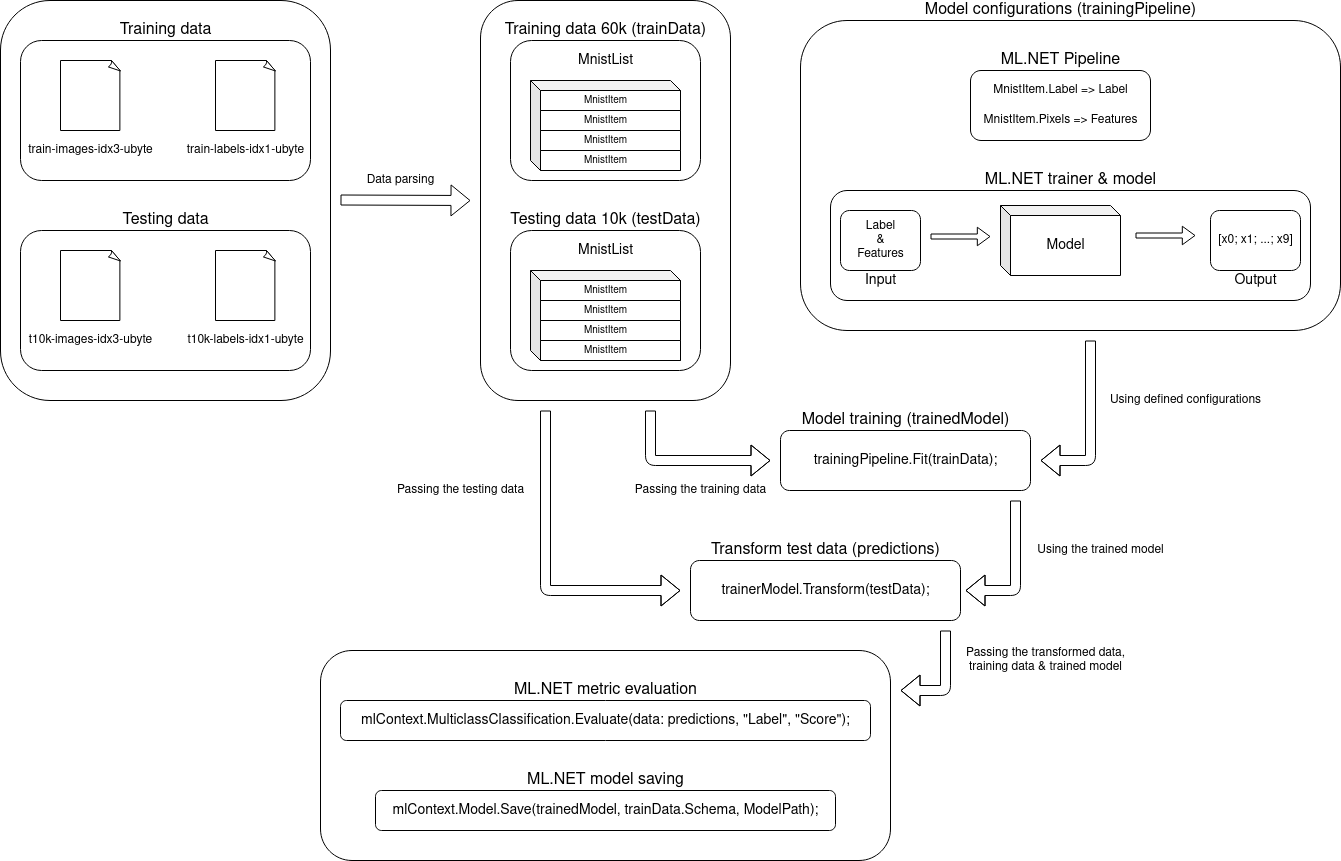
\includegraphics[width=15cm]{VPL-ML.png}
        \caption{ML modeļa trennēšanas diagramma}
        \label{ml:train}
    \end{figure}
